\documentclass[spanish,12pt,letterpapper]{article}
\usepackage{babel}
\usepackage[utf8]{inputenc}
\usepackage{graphicx}
\usepackage{hyperref}
\begin{document}
	\begin{titlepage}
		\begin{center}
			
\includegraphics[width=0.6\textwidth]{../logoUnADM}~\\[1cm] 
			\textsc{Universidad Abierta y a Distancia de México}\\[0.8cm]
			\textsc{Desarrollo de Software}\\[1.8cm]
			
			\textbf{ \Large Actividad 2. Administración y jerarquía de la memoria}\\[3cm]
			
			Diego Antonio Plascencia Lara\\ ES1421004131 \\[0.4cm]
			Facilitador(a): NORA CHIRINO MARTINEZ\\
			Asignatura: Programación de sistemas operativos\\
			Grupo: DS-DPSO-1601-B2-005 \\
			Unidad: I \\
			
			\vfill México D.F\\{\today}
			
		\end{center}
	\end{titlepage}
	
	\section{MindMap}
	\begin{center}
	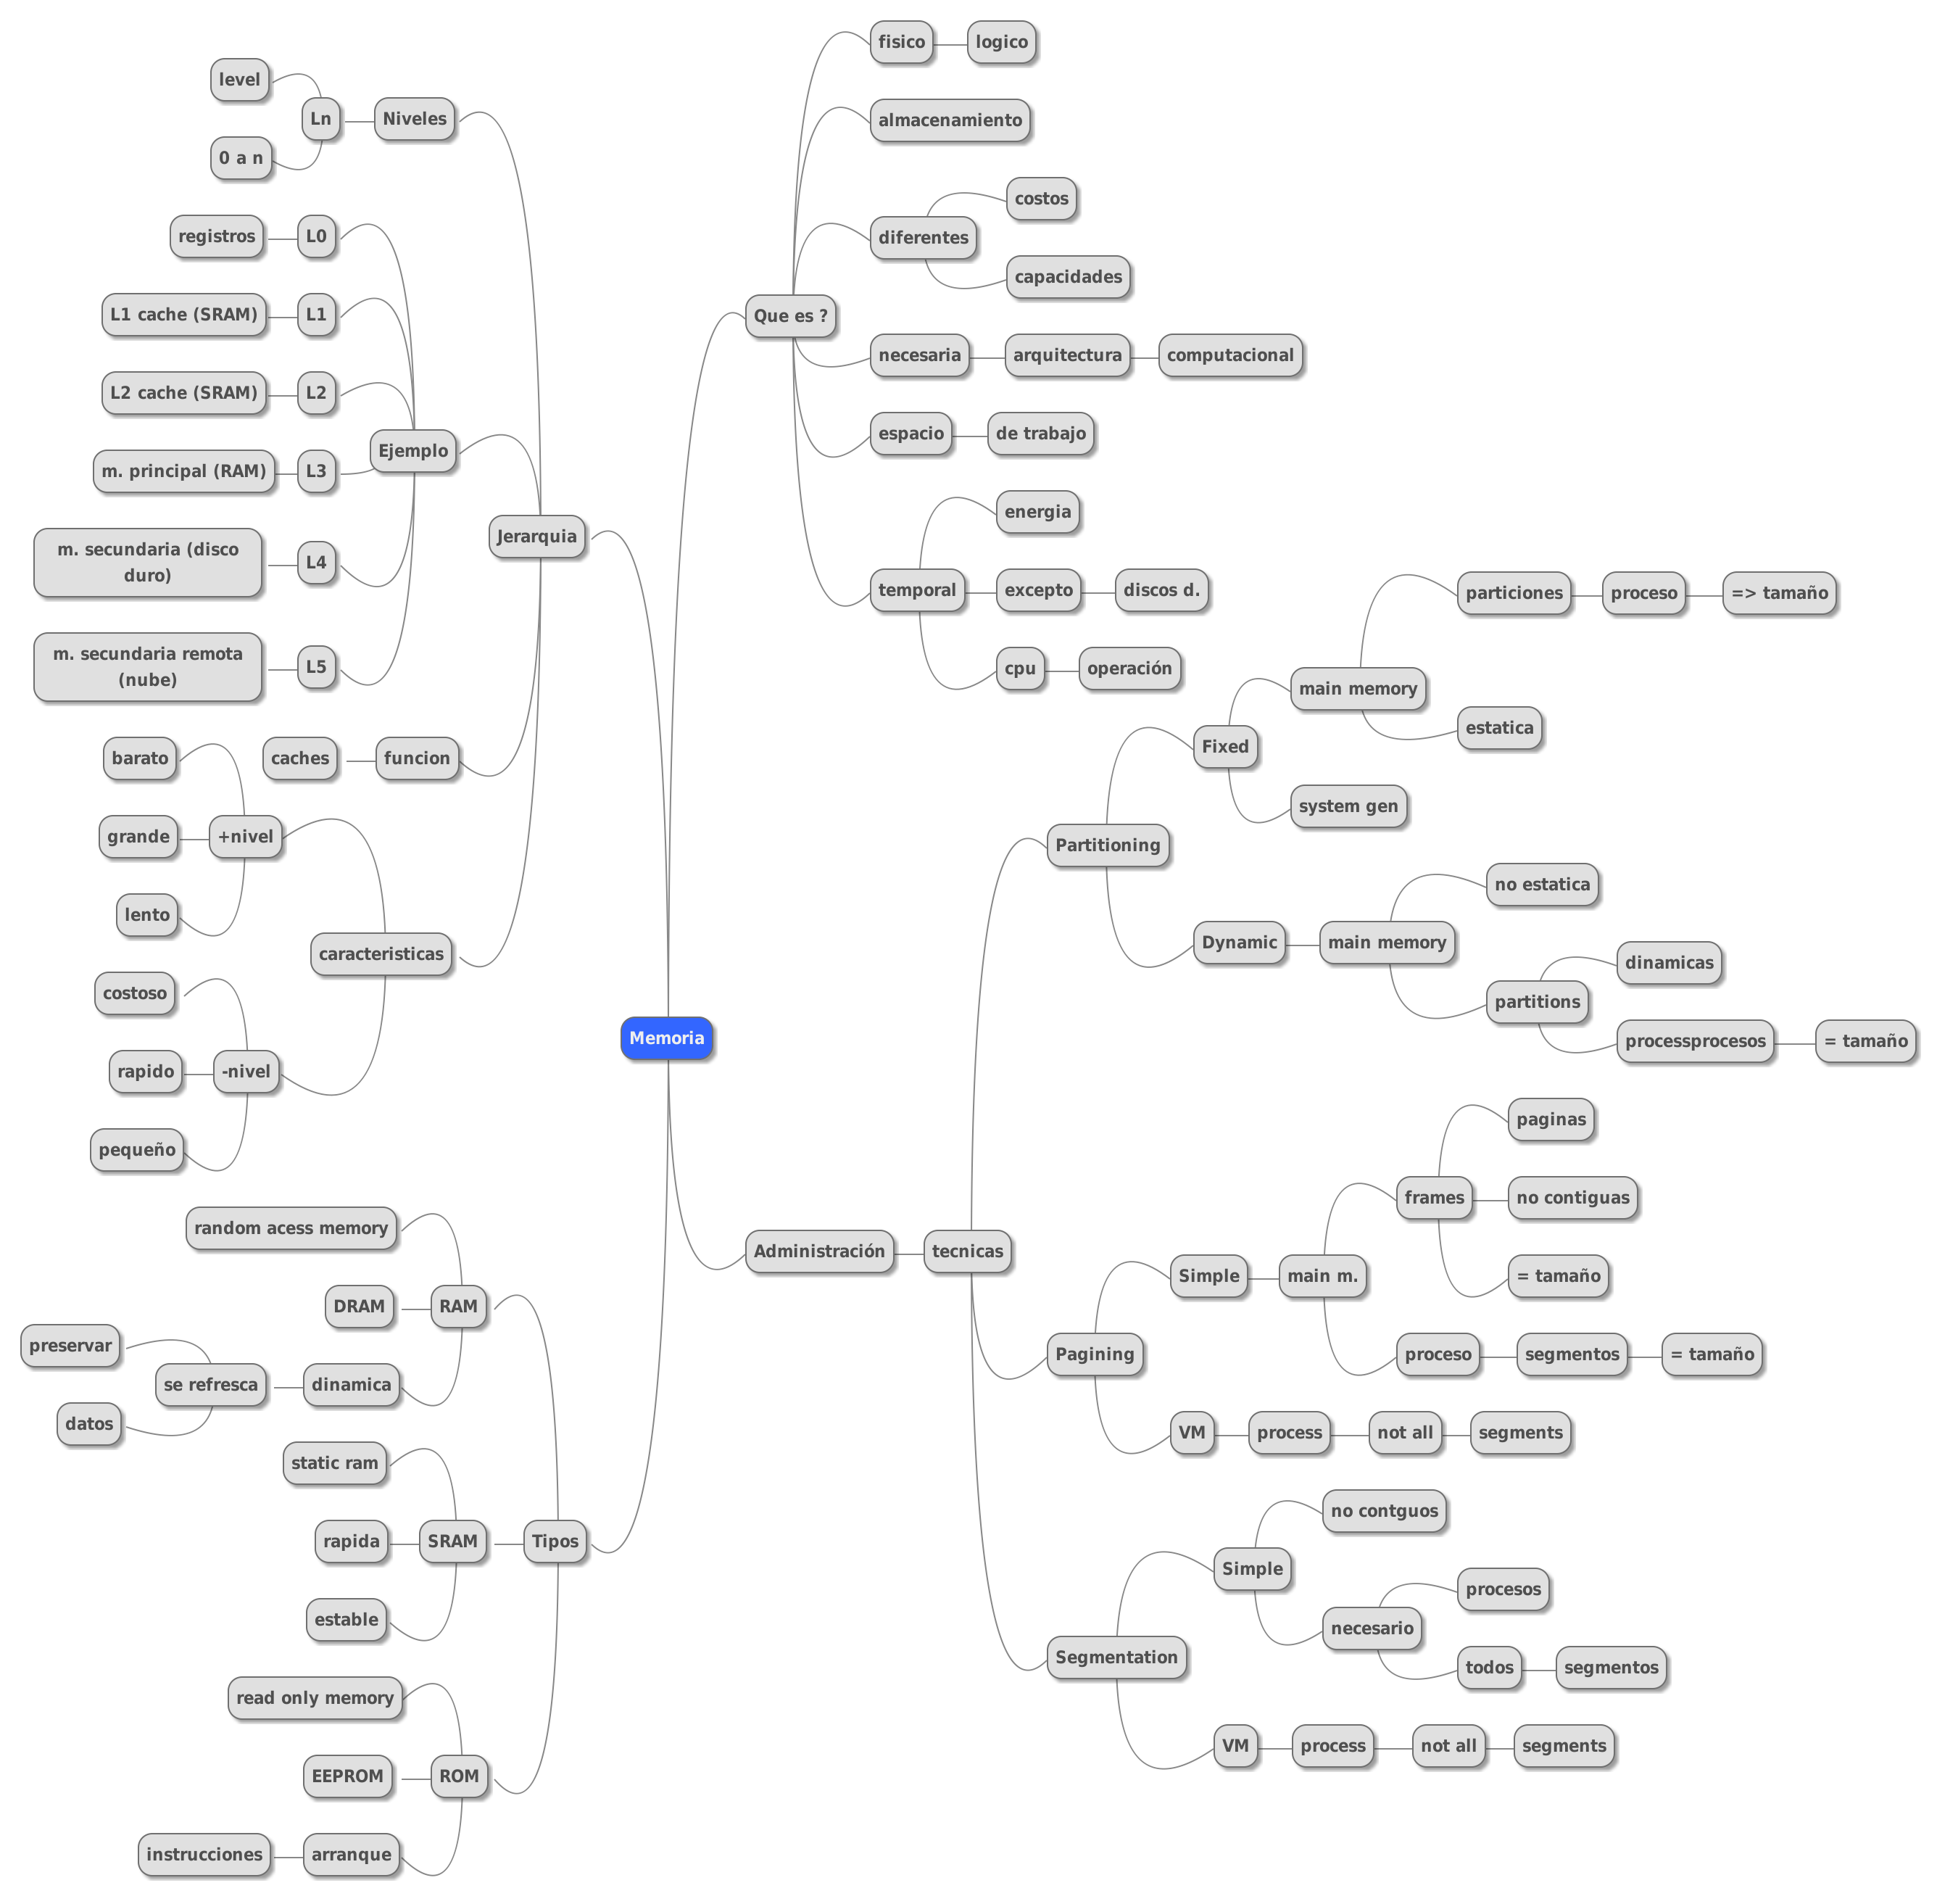
\includegraphics[width=0.8\textwidth]{./mindmap}~\\[1cm] 
	\end{center}
	\section{Memoria}
	La memoria es un espacio de trabajo para el CPU, este es temporal, y es donde el procesador almacena y ejecuta las instrucciones.
	
	Hay diferentes tipo de memoria y estas varían en costos, velocidad de escritura-lectura, capacidad, las mas conocidas son:
	
	\begin{itemize}
	\item \textbf{ROM.} Read-Only Memory, es una memoria de solo lectura, o de no muy común o difícil escritura, en este normalmente se almacena una serie de instrucciones que hacen ``arrancar'' el equipo, esta memoria no es volátil (conserva los datos aún sin energía eléctrica), la mas conocida es la EEPROM (Eelectrically Erasable Programmable ROM).
	
	\item \textbf{DRAM.} Dynamic Random Access Memory, o mas conocida como solo RAM, es la memoria principal de una computadora, en esta se pueden almacenar una cantidad considerada de bits para poder ejecutar programas, es dinámica lo cual al no haber energía eléctrica se pierde la información, así como tambien debe estarse ``refrescando'' la información (leer y reescribir) para que no se pierda al bajar el voltaje de los capacitores.
	
	\item \textbf{SRAM.} Static RAM, es un tipo de memoria utilizado normalmente en el procesador como memorias caché, estas memorias son de nivel 1, 2 y/o 3 (dependiendo del procesador), por lo que son un intermedio entre los registros del CPU y la RAM.
    \end{itemize}	 
	
	\section{Técnicas de Administración de Memoria}
	\paragraph{Fixed Partitioning.} Se fragmenta la memoria en tamaños fijos, y un proceso debe almacenarse en uno de estos fragmentos pero debe ser mas grande o de igual tamaño.
	
	\paragraph{Dynamic Partitioning.} Similar a la anterior pero los fragmentos se hacen dinámicamente para no dejar espacio sin usar.
	
	\paragraph{Simple Pagining.} Se crean distintas ``páginas'' de igual tamaño en la memoria y un proceso debe almacenarse en una o mas paginas y cargar las que sean necesarias de un proceso, estas pueden almacenarse en paginas continuas o no.
	
	\paragraph{Virtual-Memory Pagining.} Similar a la anterior, pero las paginas de un proceso van cargándose dinamicamente conforme se necesitan.
	
	\paragraph{Simple Segmentation.} Un proceso se segmenta en diferentes partes y estas se cargan en las diferentes particiones de la memoria, para que un proceso se cargue completamente deben cargarse todas sus partes. No necesitan ser contiguas.
	
	\paragraph{Virtual-Memory Segmentation.}	 Similar a la anterior pero las partes pueden cargarse dinamicamente conforme se van necesitando.
	
	\begin{center}
	\begin{tabular}{|p{4cm}|p{4cm}|p{4cm}|}
	\hline
	\textbf{Técnica} & \textbf{Ventajas} & \textbf{Inconvenientes}\\
	\hline
	Fixed Partitioning & Simple de implementar, satisface los requerimientos para un sistema operativo pequeño & Naturalmente hay memoria inutilizada y usada ineficientemente así como un numero máximo de procesos fijo  \\
	\hline
	Dynamic Partitioning & No tiene fragmentación lo que tiene un mejor uso de la memoria & Ineficiente uso del procesador debido a la necesidad de compactar para el contador de fragmentación externa.\\
	\hline
	Simple Paging & No fragmentación externa & Pequeño monto de fragmentación externa.\\
	\hline
	Virtual-Memory Pagining & No fragmentación externa, alto grado de programación, gran espacio de memoria virtual & Alta complejidad de administración de la memoria.\\
	\hline
	Virtual-Memory Segmentation & No fragmentación externa, alto grado de programación, gran espacio de memoria virtual soporte de protección y compartir & Alta complejidad de administración de la memoria.\\
	\hline
	\end{tabular}
	\end{center}	
	
	\pagebreak
	\section{Jerarquía de Memoria}
	La jerarquía entre las memorias de una computadora esta dada por niveles que van del 0 al n, siendo el nivel 0 los registros del CPU.\\
	
	A mayor nivel, mayor es el costo y la velocidad de trasferencia de datos pero menor es la densidad (capacidad de almacenamiento), esto quiere decir que los registros del CPU tienen la mayor jerarquía al ser la memoria a la cual recurre el procesador para leer y ejecutar.\\
	
	La jerarquía sirve para poder dar un mejor rendimiento a los programas, ya que cada una sirve de caché a el siguiente nivel en la jerarquía, es decir que para cada k, el dispositivo mas rápido y pequeño en el nivel k, sirve de caché a el dispositivo más lento y grande en el nivel k+1. Por ejemplo, el cache L2 sirve de cache a la memoria RAM.\\
	
	\begin{center}
	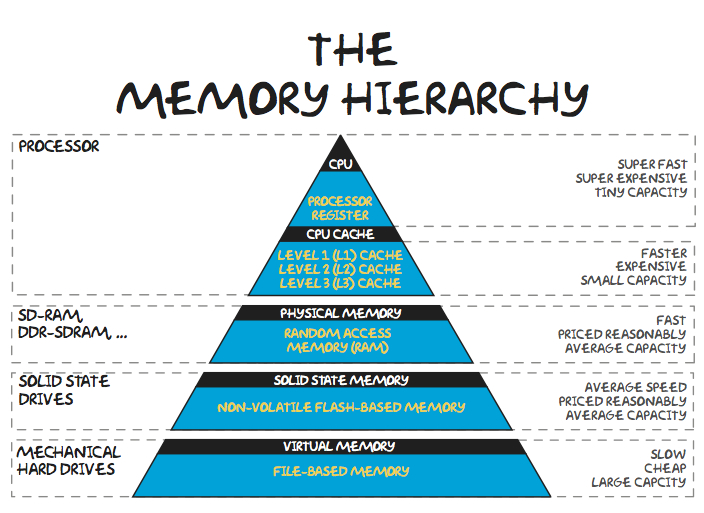
\includegraphics[width=0.8\textwidth]{./memh}~\\[1cm] 
	\end{center}
	
	\section{Conclusión}
	Es importante entender las jerarquías de la memoria por que nos permite conocer como se organiza y entender conceptos como el caché, así podemos tener conocimientos para poder hacer software mas eficiente. De igual manera es importante conocer las técnicas de administración de memoria, por la misma razón, conocer como funciona la memoria y como nuestro software es ejecutado y podemos hacer el manejo de memoria de un software mas eficiente. 
	
	\pagebreak
	\begin{thebibliography}{9}
		\bibitem{OperatingSystemConcepts} Silberschatz, A. Baer P. Gagne G.(2013).
		\emph{Operating System Concepts}. USA: Wiley.
		\bibitem{memherarchy} Bryant Randy \& O’Hallaron Dave.
		\emph{The Memory Hierarchy}. USA: Carnegie Mellon University.
	\end{thebibliography}
	
\end{document}